\documentclass[a4paper,12pt]{article}
\usepackage{fontspec}
\setmainfont{Times New Roman}
\setsansfont{Arial}
\setmonofont{Courier New}

% Manual Vietnamese localization (since babel-vietnamese is missing)
\renewcommand{\contentsname}{Mục lục}
\renewcommand{\listfigurename}{Danh sách hình vẽ}
\renewcommand{\listtablename}{Danh sách bảng}
\renewcommand{\figurename}{Hình}
\renewcommand{\tablename}{Bảng}
\renewcommand{\refname}{Tài liệu tham khảo}
\usepackage[ddmmyyyy]{datetime}
\renewcommand{\dateseparator}{/}
\usepackage{graphicx}
\usepackage[colorlinks=true, linkcolor=black, urlcolor=blue, citecolor=black]{hyperref}
\usepackage{listings}
\usepackage{xcolor}
\usepackage{float}
\usepackage{geometry}
\usepackage{tabularx}
\usepackage{amsmath}
\usepackage{fancyhdr}

% Page Geometry
\geometry{
 a4paper,
 total={170mm,257mm},
 left=20mm,
 top=20mm,
 headheight=15pt,
}

% Header Configuration
\pagestyle{fancy}
\fancyhf{}
\fancyhead[L]{dtn\_elib}
\fancyhead[R]{\thepage}
\renewcommand{\headrulewidth}{0.4pt}

% Code Listing Style
\definecolor{codegray}{rgb}{0.5,0.5,0.5}
\definecolor{codepurple}{rgb}{0.58,0,0.82}
\definecolor{backcolour}{rgb}{0.95,0.95,0.92}

% Custom colors for highlighting
\definecolor{darkblue}{rgb}{0.0,0.2,0.6}
\definecolor{darkgreen}{rgb}{0.0,0.5,0.0}
\definecolor{darkred}{rgb}{0.7,0.0,0.0}

\lstdefinestyle{mystyle}{
    backgroundcolor=\color{backcolour},   
    commentstyle=\color{codegray},
    keywordstyle=\color{magenta},
    numberstyle=\tiny\color{codegray},
    stringstyle=\color{codepurple},
    basicstyle=\ttfamily\footnotesize,
    breakatwhitespace=false,         
    breaklines=true,                 
    captionpos=b,                    
    keepspaces=true,                 
    numbers=left,                    
    numbersep=5pt,                  
    showspaces=false,                
    showstringspaces=false,
    showtabs=false,                  
    tabsize=2
}
\lstdefinelanguage{json}{
    basicstyle=\normalfont\ttfamily,
    numbers=left,
    numberstyle=\scriptsize,
    stepnumber=1,
    numbersep=8pt,
    showstringspaces=false,
    breaklines=true,
    frame=lines,
    backgroundcolor=\color{backcolour},
    literate=
     *{0}{{{\color{blue}0}}}{1}
      {1}{{{\color{blue}1}}}{1}
      {2}{{{\color{blue}2}}}{1}
      {3}{{{\color{blue}3}}}{1}
      {4}{{{\color{blue}4}}}{1}
      {5}{{{\color{blue}5}}}{1}
      {6}{{{\color{blue}6}}}{1}
      {7}{{{\color{blue}7}}}{1}
      {8}{{{\color{blue}8}}}{1}
      {9}{{{\color{blue}9}}}{1}
      {:}{{{\color{red}{:}}}}{1}
      {,}{{{\color{red}{,}}}}{1}
      {\{}{{{\color{blue}{\{}}}}{1}
      {\}}{{{\color{blue}{\}}}}}{1}
      {[}{{{\color{blue}{[}}}}{1}
      {]}{{{\color{blue}{]}}}}{1},
}
\lstset{style=mystyle}

% Metadata
\title{\textbf{BÁO CÁO TỔNG HỢP DỰ ÁN CUỐI KỲ} \\ \Large HỆ THỐNG THƯ VIỆN ĐIỆN TỬ PHÂN TÁN (E-LIBRARY)}
\author{\textbf{Nhóm Sinh viên:} \\ Nguyễn Tiến Đạt - 835151465 \\ Đặng Trung Kiên - 835151466 \\ Nguyễn Diệp Linh - 835151467}
\date{Ngày 05 tháng 01 năm 2026}

\begin{document}

\maketitle

\vspace{1cm}
\begin{center}
{\large \textbf{Link Dự án:}} \\
\vspace{0.3cm}
{\large \url{https://bitbucket.org/dtn__ntd/elib/src/dtn_elib/}}
\end{center}

\tableofcontents
\newpage

\listoffigures
\newpage

\listoftables
\newpage

% -------------------------------------------------------------------
\section{Giới thiệu \& Mục tiêu Hệ thống}

{\color{darkblue}\textbf{E-Library}} là hệ thống thư viện kỹ thuật số phân tán, quản lý toàn diện vòng đời sách (Vật lý \& Điện tử) trên quy mô lớn.

\subsection{Mục tiêu Chính}
\begin{itemize}
    \item {\color{darkblue}\textbf{Sharded Cluster}}: Phân tán dữ liệu users/loans theo địa lý (Hà Nội, Hải Phòng, Đà Nẵng).
    \item {\color{darkgreen}\textbf{High Availability}}: Đảm bảo failover tự động trong 2-3s nhờ Replica Set.
    \item {\color{darkblue}\textbf{Phỏng theo Kinh doanh số}}: Mô hình membership hiện đại với tính năng Sách điện tử, Ví và Gói VIP.
\end{itemize}

\subsection{Phạm vi Dự án (Scope)}
Hệ thống tập trung giải quyết các bài toán cốt lõi của thư viện hiện đại:
\begin{itemize}
    \item \textbf{Quản lý Sách}: Vòng đời từ nhập kho, đánh mã vạch (Barcode) đến thanh lý.
    \item \textbf{Lưu thông (Circulation)}: Quy trình Mượn - Trả - Gia hạn tự động.
    \item \textbf{Thương mại}: Tích hợp ví điện tử giả lập để mua gói VIP đọc sách không giới hạn.
\end{itemize}

% -------------------------------------------------------------------
\section{Công nghệ \& Tổ chức Mã nguồn}

\subsection{Công nghệ Sử dụng}
\begin{table}[H]
\centering
\begin{tabularx}{\textwidth}{|l|X|X|}
\hline
\textbf{Thành phần} & \textbf{Công nghệ} & \textbf{Mục đích} \\
\hline
\textbf{Frontend} & ReactJS, Vite, TailwindCSS & Giao diện người dùng (SPA), Components hóa. \\
\hline
\textbf{Backend} & Go (Golang) v1.23 & API Server hiệu năng cao, xử lý concurrency tốt. \\
\hline
\textbf{Web Framework} & Gin-Gonic & Router nhanh, Middleware (Auth, CORS). \\
\hline
\textbf{Database} & MongoDB 7.0 (Sharded) & Lưu trữ phân tán, Text Search, Aggregation. \\
\hline
\textbf{Auth} & JWT & Xác thực không trạng thái (Stateless). \\
\hline
\textbf{Infrastructure} & Docker, Docker Compose & Container hóa toàn bộ môi trường Dev/Prod. \\
\hline
\end{tabularx}
\caption{Danh sách công nghệ sử dụng}
\end{table}

\subsection{Cấu trúc Dự án}
Dự án được tổ chức theo mô hình \textbf{Monorepo}:

\begin{lstlisting}[language=bash, caption=Cây thư mục dự án]
elib/
|-- client/                 # Frontend ReactJS
|   |-- src/components/     # UI Reusable Components
|   |-- src/pages/          # Cac man hinh chinh
|   |-- src/context/        # AuthContext
|-- server/                 # Backend Go
|   |-- main.go             # Entry point
|   |-- config/             # DB Connectivity
|   |-- controllers/        # Business Logic
|   |-- models/             # Data Schema
|-- scripts/                # Utility Scripts (Seed, Bench)
|-- tests/                  # Integration Tests
|-- deploy/                 # Sharding Scripts
|-- docs/                   # Documentation
\end{lstlisting}

\subsection{Tổ chức Docker}
\begin{itemize}
    \item \textbf{Backend}: Sử dụng \texttt{Air} để Hot-reload.
    \item \textbf{Frontend}: Mount volume để HMR (Hot Module Replacement).
    \item \textbf{Database Cluster}: 9 containers MongoDB được khởi tạo và cấu hình tự động bởi \texttt{init.sh}, chạy hoàn toàn trong mạng riêng \texttt{elib-net}.
\end{itemize}

% -------------------------------------------------------------------
\section{Kiến trúc Phân tán (Infrastructure)}

\subsection{Sơ đồ Hạ tầng \& Các Node Phân tán}
Hệ thống gồm 11 Container phối hợp hoạt động.

\begin{figure}[H]
    \centering
    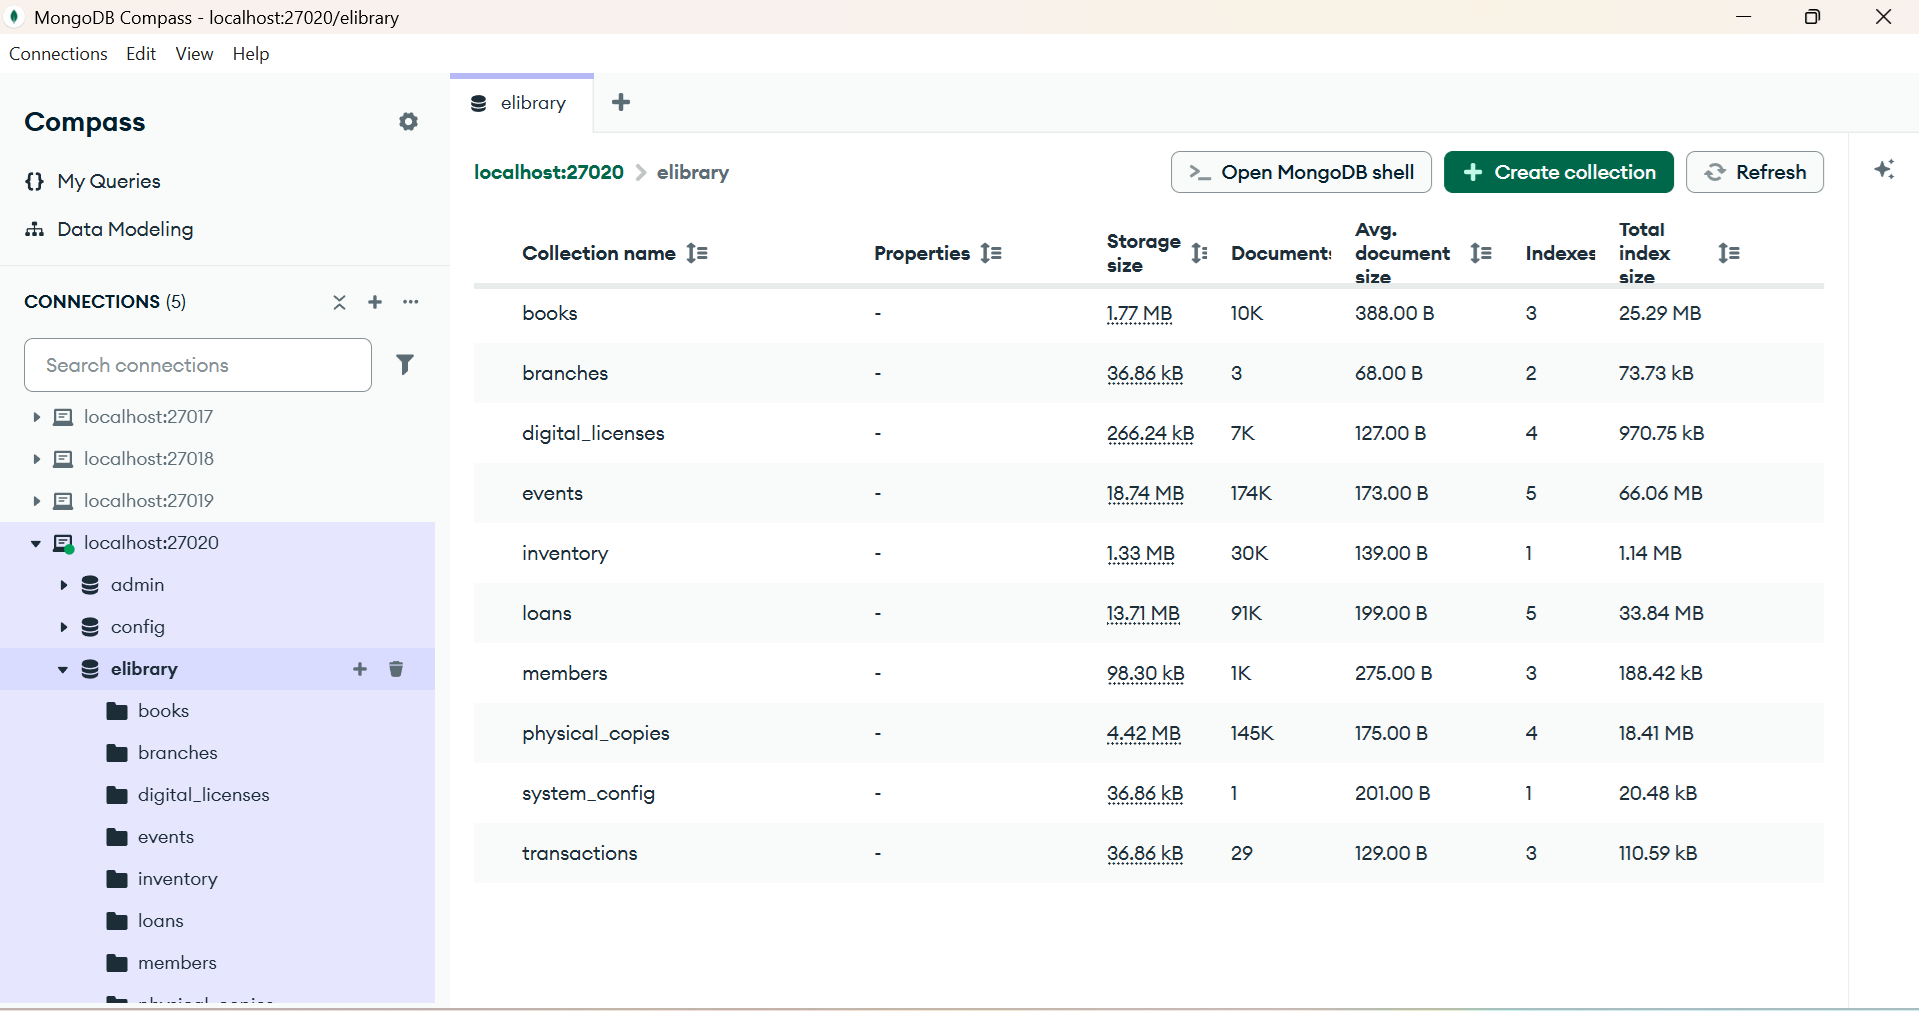
\includegraphics[width=0.9\linewidth]{img/mongo.png}
    \caption{Kiến trúc Sharding Logic MongoDB}
\end{figure}

\begin{table}[H]
\centering
\begin{tabular}{|l|l|l|l|}
\hline
\textbf{Role} & \textbf{Container} & \textbf{Port} & \textbf{Mô tả} \\
\hline
\textbf{Router} & \texttt{mongos1} & :27020 & Cổng tiếp nhận truy vấn. \\
\hline
\textbf{Config} & \texttt{cfg1-3} & :27117 & Replica Set lưu Metadata. \\
\hline
\textbf{Shard 1} & \texttt{hn1} (HN) & :27017 & \textbf{Primary} (Zone miền Bắc). \\
\hline
\textbf{Shard 1} & \texttt{hp1} (HP) & :27018 & \textbf{Secondary} (Failover). \\
\hline
\textbf{Shard 1} & \texttt{dn1} (DN) & :27019 & \textbf{Secondary} (Zone miền Trung). \\
\hline
\textbf{Shard 2} & \texttt{ex1, ex2} & :27217 & Zone mở rộng (Hash Sharding). \\
\hline
\end{tabular}
\caption{Danh sách Docker Containers}
\end{table}

\begin{figure}[H]
    \centering
    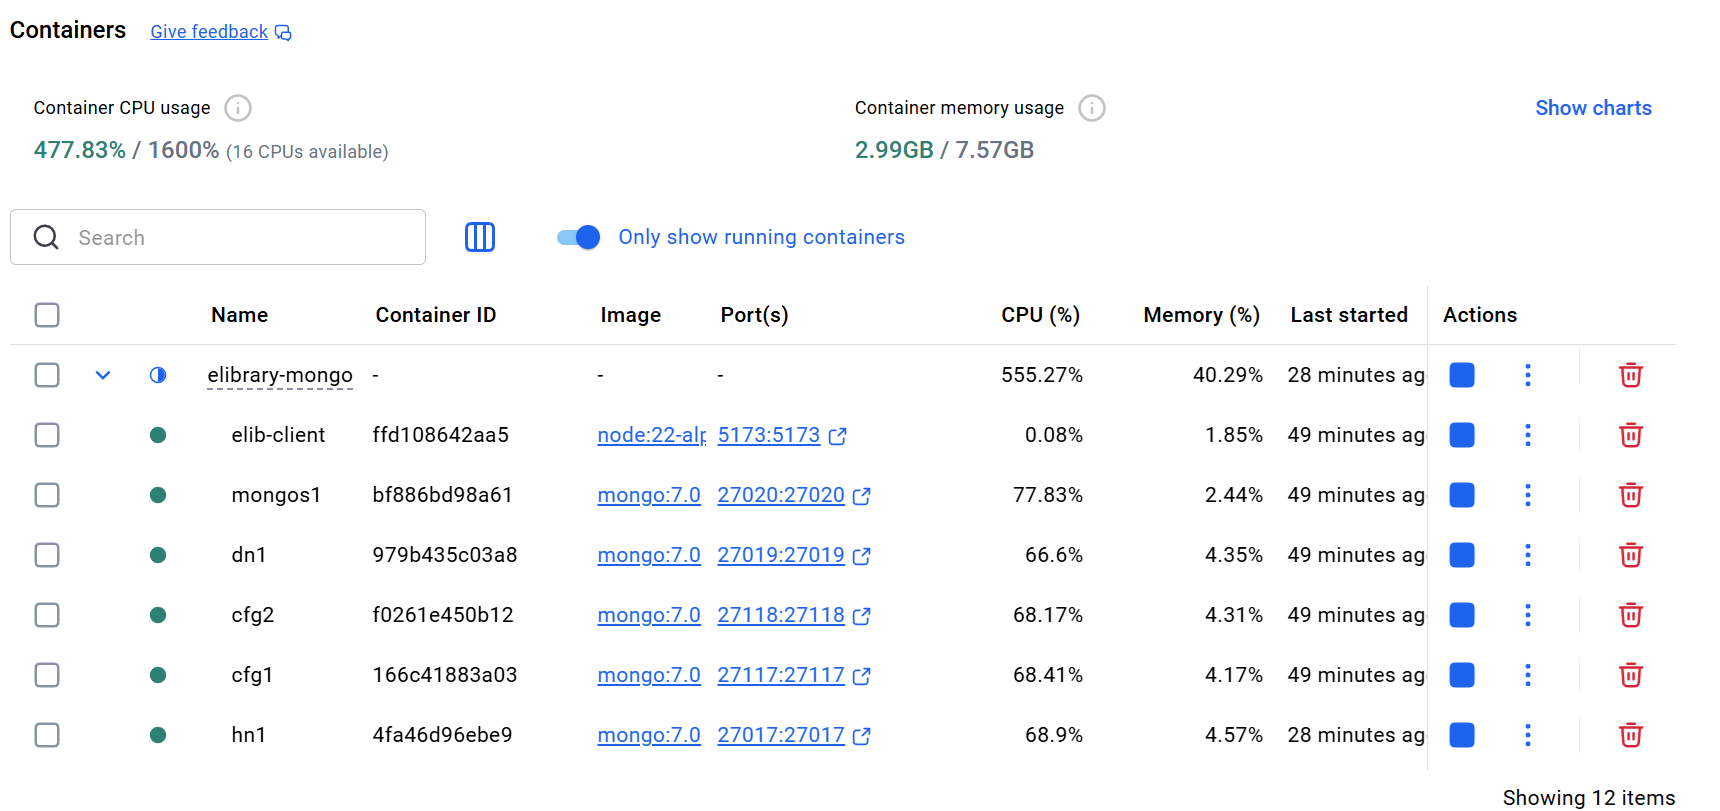
\includegraphics[width=0.9\linewidth]{img/docker.png}
    \caption{Trạng thái Container thực tế trong Docker}
\end{figure}

\begin{figure}[H]
    \centering
    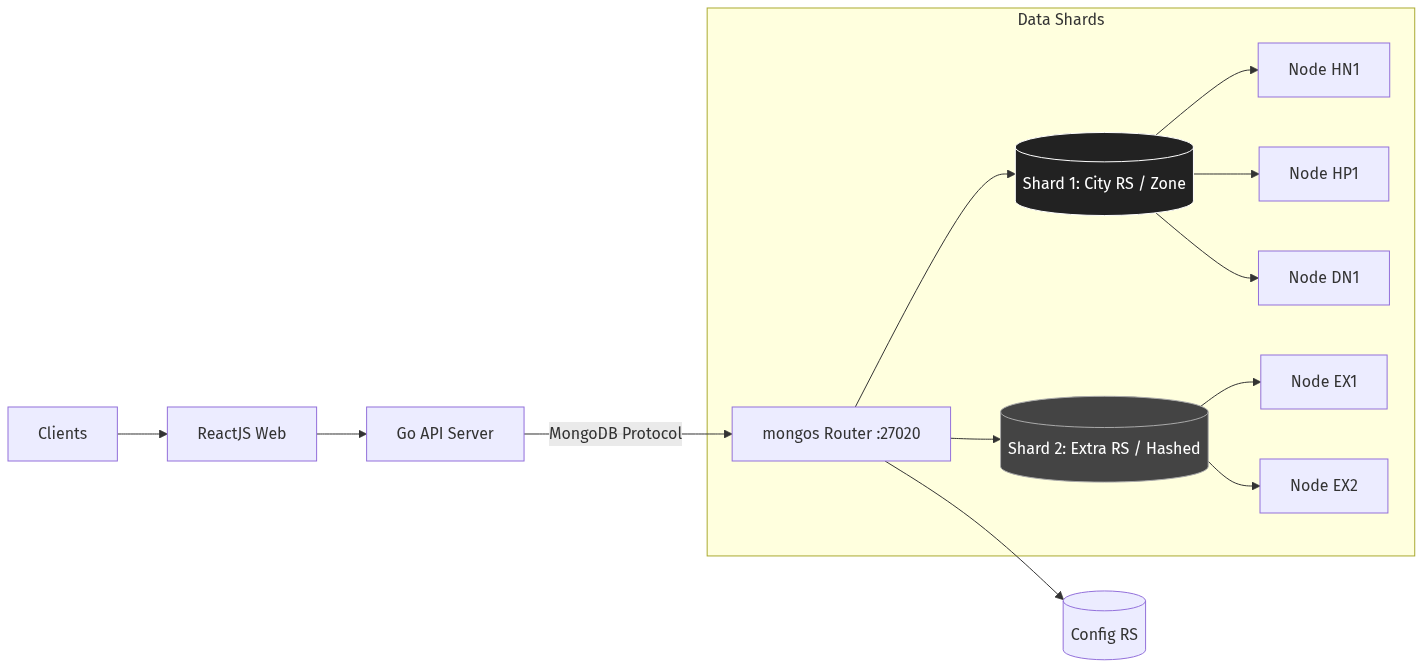
\includegraphics[width=1.0\linewidth]{img/chart_arch.png}
    \caption{Sơ đồ Luồng dữ liệu (Data Flow)}
\end{figure}

\subsection{Chứng minh Phân tải (Sharding Verification)}
\begin{itemize}
    \item \textbf{Shard \texttt{rsCity}}: Chứa toàn bộ dữ liệu chính (\texttt{loans}, \texttt{members}) do cấu hình Zone Sharding tập trung vào tính địa phương (Data Locality).
    \item \textbf{Shard \texttt{rsExtra}}: Ở trạng thái chờ (Standby), sẵn sàng nhận chunk khi dữ liệu mỗi vùng vượt quá ngưỡng.
\end{itemize}

\subsection{Nguyên lý Thiết kế}
\begin{enumerate}
    \item \textbf{Phân tán}: Tách biệt Router - Config - Shard để đảm bảo Single Responsibility và khả năng mở rộng ngang (Scale-out).
    \item \textbf{Zone Sharding}: Tối ưu hóa độ trễ (Latency) dựa trên tính địa phương của dữ liệu thư viện (Người dùng HN truy vấn Server HN).
    \item \textbf{Search Engine}: Sử dụng \textbf{Inverted Index} và cơ chế Scatter-Gather để tìm kiếm song song trên toàn cụm.
\end{enumerate}

% -------------------------------------------------------------------
\section{Thiết kế Dữ liệu \& API}

\subsection{Lược đồ Quan hệ (ERD)}
Mô tả mối quan hệ giữa các Collection trong hệ thống.
\begin{figure}[H]
    \centering
    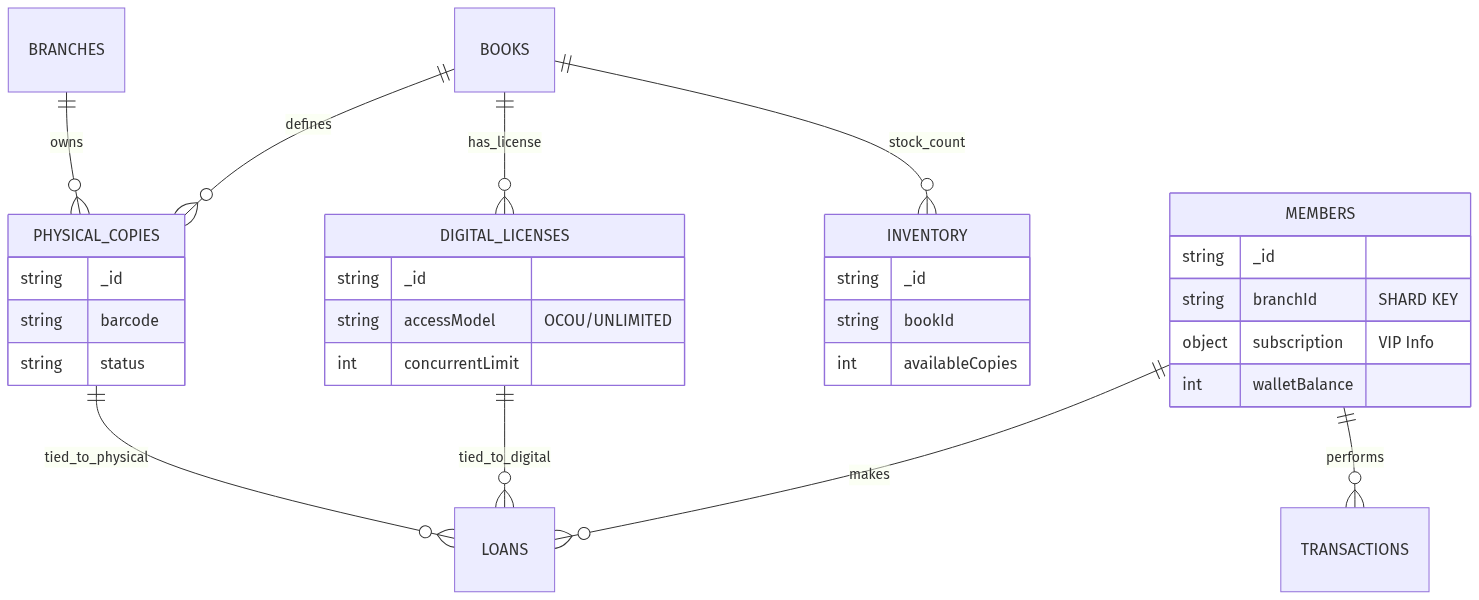
\includegraphics[width=0.9\linewidth]{img/chart_erd.png}
    \caption{Entity Relationship Diagram (Mermaid)}
\end{figure}

\subsection{API Endpoints}
\begin{table}[H]
\centering
\begin{tabularx}{\textwidth}{|l|l|l|X|}
\hline
\textbf{Module} & \textbf{Method} & \textbf{Endpoint} & \textbf{Mô tả} \\
\hline
Auth & POST & /api/auth/login & Đăng nhập lấy JWT. \\
\hline
Books & GET & /api/books & Tìm kiếm sách (Filter). \\
\hline
Loans & POST & /api/loans/borrow & Mượn sách (Check Quota). \\
\hline
Wallet & POST & /api/wallet/topup & Nạp tiền VIP. \\
\hline
\end{tabularx}
\caption{Các API chính}
\end{table}

\textbf{Ví dụ JSON Response (Success):}
\begin{lstlisting}[language=json]
// GET /api/books?limit=1
{
  "data": [
    {
      "id": "60a7...",
      "title": "Clean Code",
      "price": 150000,
      "available": true
    }
  ],
  "meta": {
    "total": 1050,
    "page": 1
  }
}
\end{lstlisting}

\subsection{Chi tiết Implement Tìm kiếm (Search Logic)}
Hệ thống hỗ trợ 2 cơ chế tìm kiếm trong \texttt{book\_controller.go}:

\textbf{1. Regex Search (Flexible)}
\begin{lstlisting}[language=Go]
if search != "" {
    matchStage["$or"] = []bson.M{
        {"title": bson.M{"$regex": search, "$options": "i"}},
    }
}
\end{lstlisting}
\textit{Nhược điểm: Quét toàn bộ bảng, chậm với dữ liệu lớn.}

\textbf{2. Text Index Search (High Performance)}
\begin{lstlisting}[language=Go]
if search != "" {
    matchStage["$text"] = bson.M{"$search": search}
}
\end{lstlisting}
Use Inverted Index, response time \textasciitilde 2ms.

% -------------------------------------------------------------------
\subsection{Cơ chế Bảo mật (Security Implementation)}
Hệ thống áp dụng các lớp bảo mật đa tầng:
\begin{enumerate}
    \item \textbf{Password Hashing}: Sử dụng thuật toán \textbf{Bcrypt} (cost factor 14) để mã hóa mật khẩu trước khi lưu vào database. Ngăn chặn tấn công Rainbow Table.
    \item \textbf{Authentication}: Sử dụng \textbf{JWT (JSON Web Token)} cho cơ chế xác thực không trạng thái (Stateless). Token chứa `userID`, `role` và `exp` (thời hạn).
    \item \textbf{Authorization (RBAC)}: Middleware kiểm soát quyền truy cập dựa trên vai trò:
    \begin{itemize}
        \item \texttt{RequireAdmin}: Chỉ cho phép Admin thao tác (vd: Nhập sách).
        \item \texttt{RequireStaff}: Cho phép Staff/Admin (vd: Xử lý mượn trả).
    \end{itemize}
    \item \textbf{VIP Auto-Check}: Middleware tự động kiểm tra ngày hết hạn VIP trong mọi request. Nếu hết hạn, hệ thống tự động giáng cấp xuống thành viên thường.
\end{enumerate}

% -------------------------------------------------------------------
\section{Luồng Nghiệp vụ (Business Flows)}

\subsection{Mượn Sách Vật Lý (Atomic Inventory Check)}
\begin{figure}[H]
    \centering
    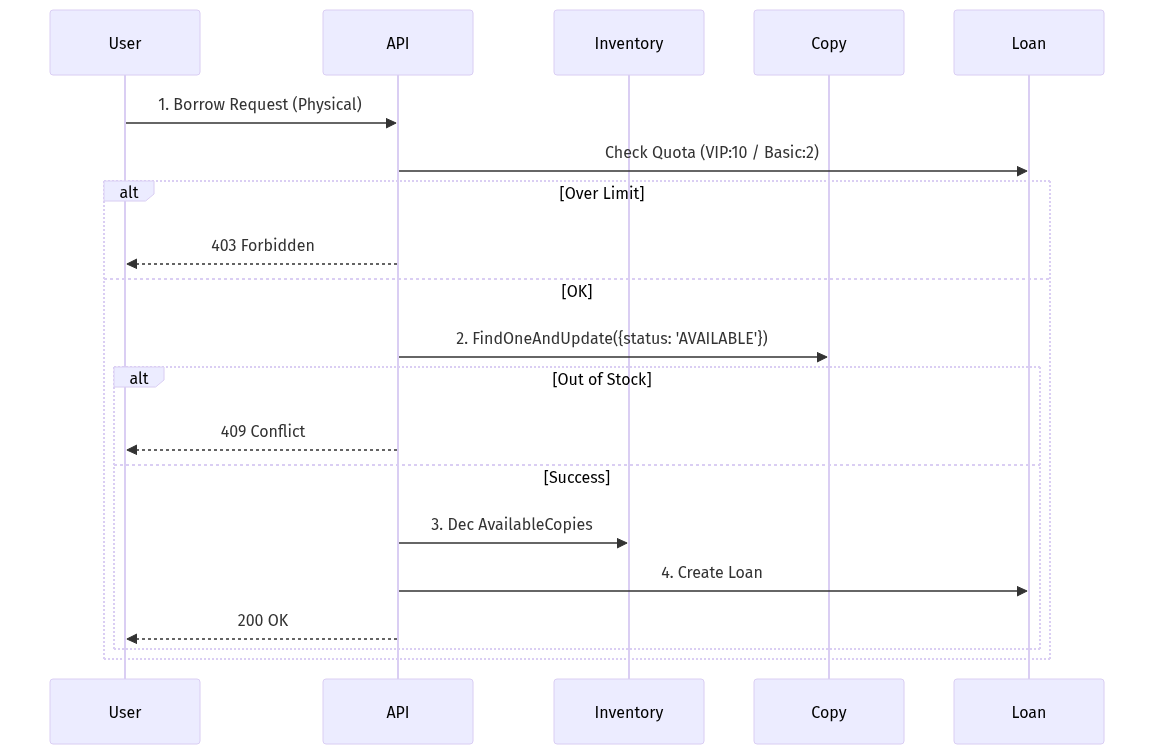
\includegraphics[width=0.9\linewidth]{img/chart_borrow.png}
    \caption{Quy trình Mượn sách Vật lý (Sequence Diagram)}
\end{figure}

\subsection{Mượn Sách Số (Digital License)}
Hệ thống phân biệt 2 mô hình bản quyền:
\begin{itemize}
    \item \textbf{OCOU (One Copy One User)}: Giới hạn số lượng bản quyền (như sách thật). Hết lượt phải chờ (Waitlist).
    \item \textbf{UNLIMITED}: Không giới hạn số người đọc. \textbf{Dành riêng cho VIP}.
\end{itemize}

\begin{figure}[H]
    \centering
    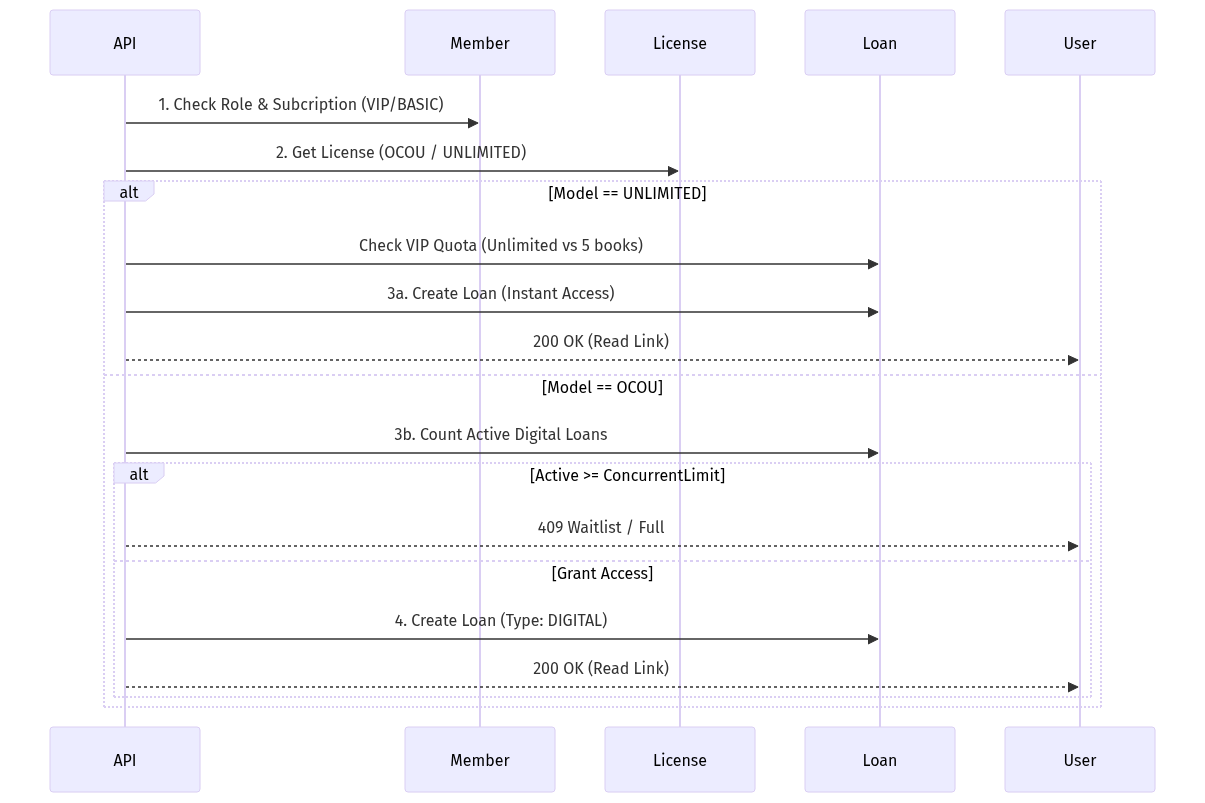
\includegraphics[width=0.9\linewidth]{img/chart_license.png}
    \caption{Quy trình Mượn sách Số (License Check)}
\end{figure}

\subsection{Mua Gói VIP (Wallet Transaction)}
\begin{figure}[H]
    \centering
    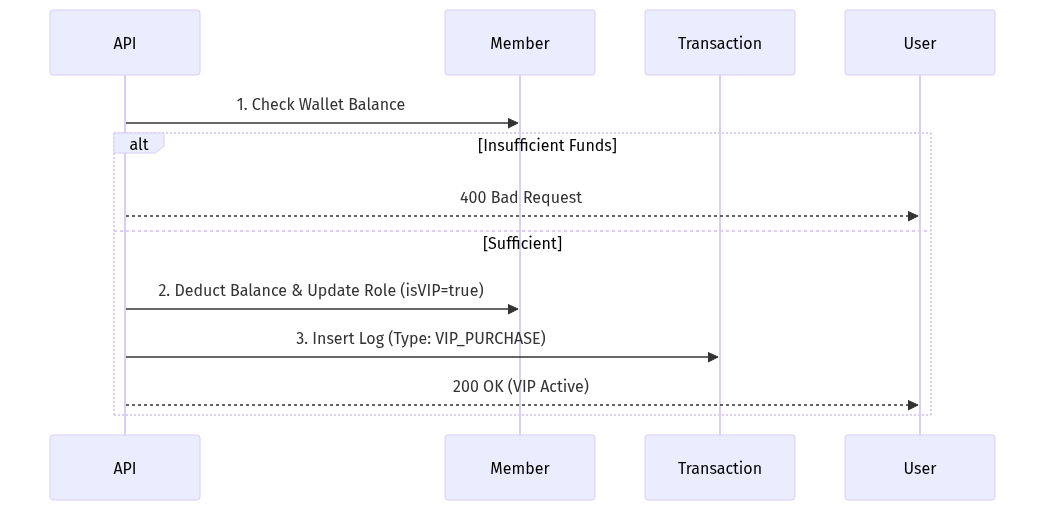
\includegraphics[width=0.8\linewidth]{img/chart_vip.png}
    \caption{Quy trình Nạp/Đăng ký VIP}
\end{figure}

% -------------------------------------------------------------------
\section{Minh chứng Giao diện (UI Views)}
Hỗ trợ đầy đủ các phân hệ từ Người dùng cuối (End-User) đến Quản trị viên (Admin/Staff).

\subsection{Trang chủ \& Membership}
Tổng quan hệ thống và các gói dịch vụ VIP.

\begin{figure}[H]
    \centering
    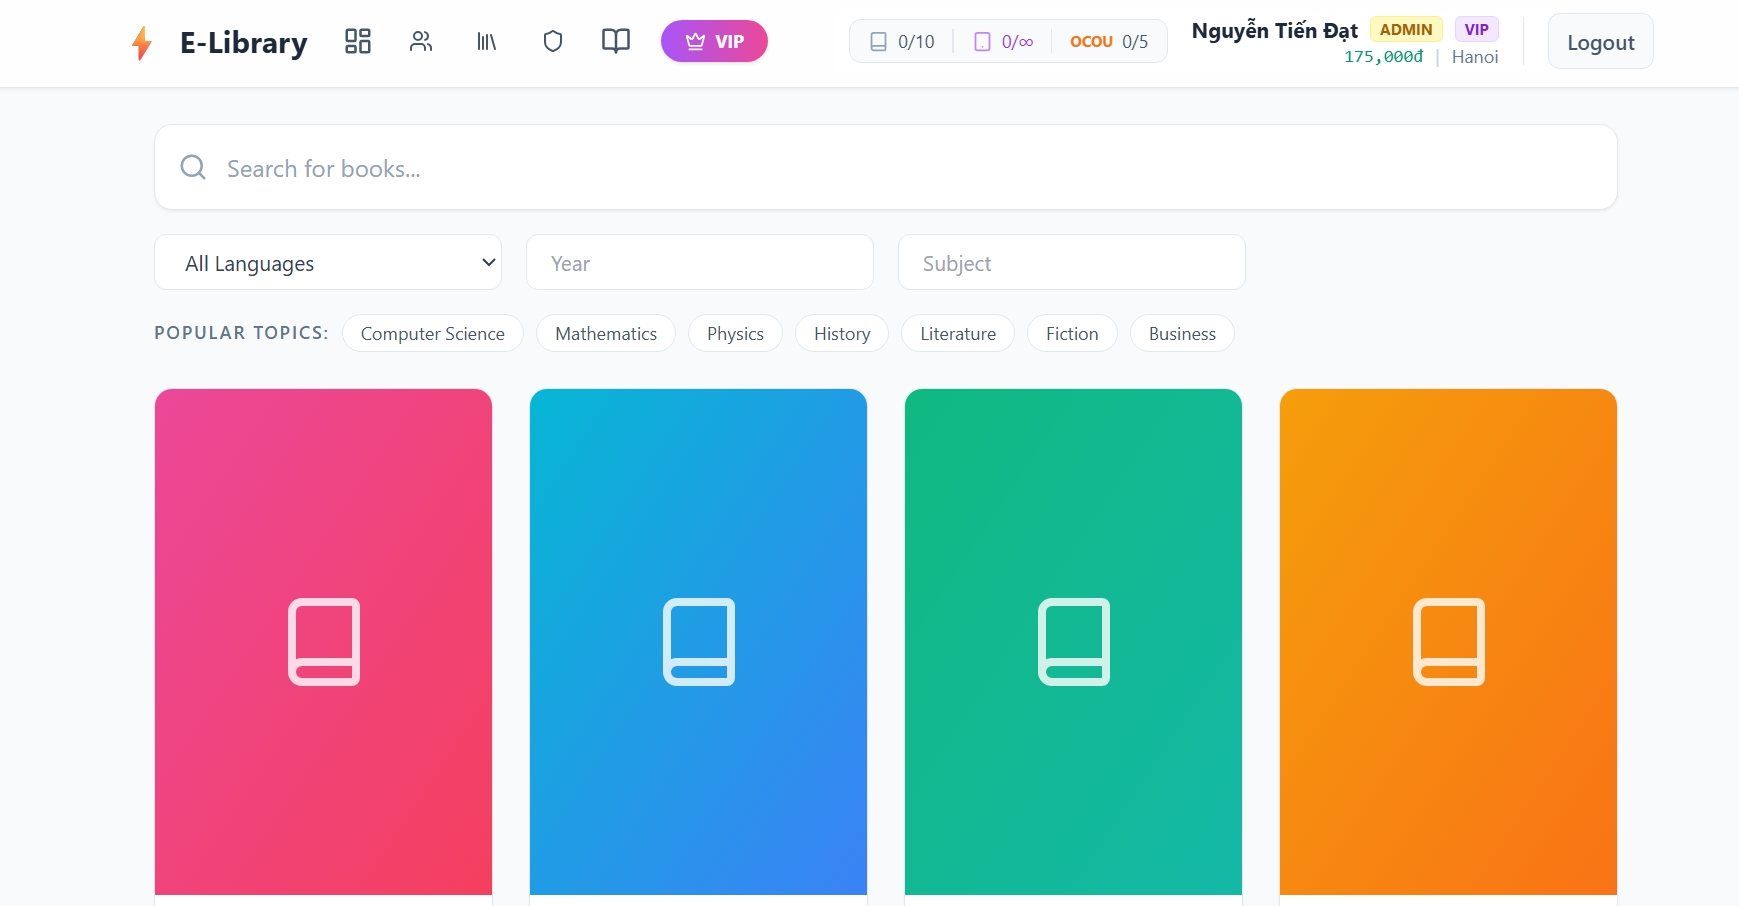
\includegraphics[width=0.8\linewidth]{img/trang_chu.jpeg}
    \caption{Giao diện Trang chủ}
\end{figure}

\begin{figure}[H]
    \centering
    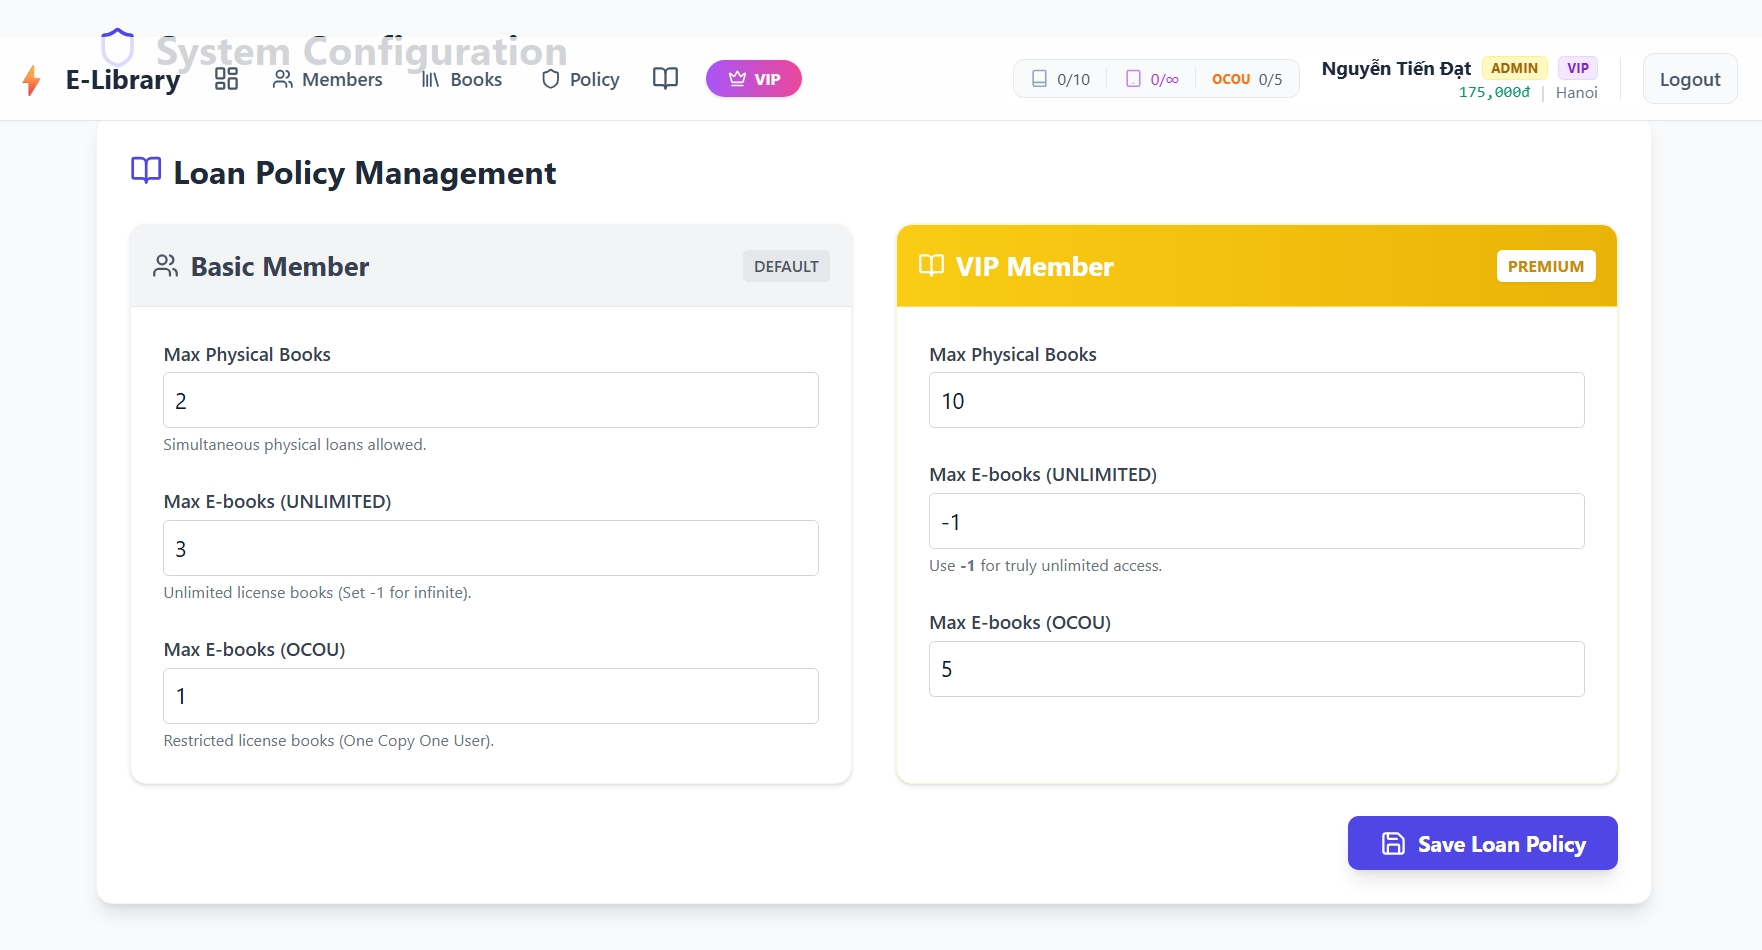
\includegraphics[width=0.8\linewidth]{img/policy_vip.jpeg}
    \caption{Chính sách và Đăng ký VIP}
\end{figure}

\subsection{Quản trị Sách \& Thành viên (Admin)}
Dành cho Admin quản lý danh mục và người dùng.

\begin{figure}[H]
    \centering
    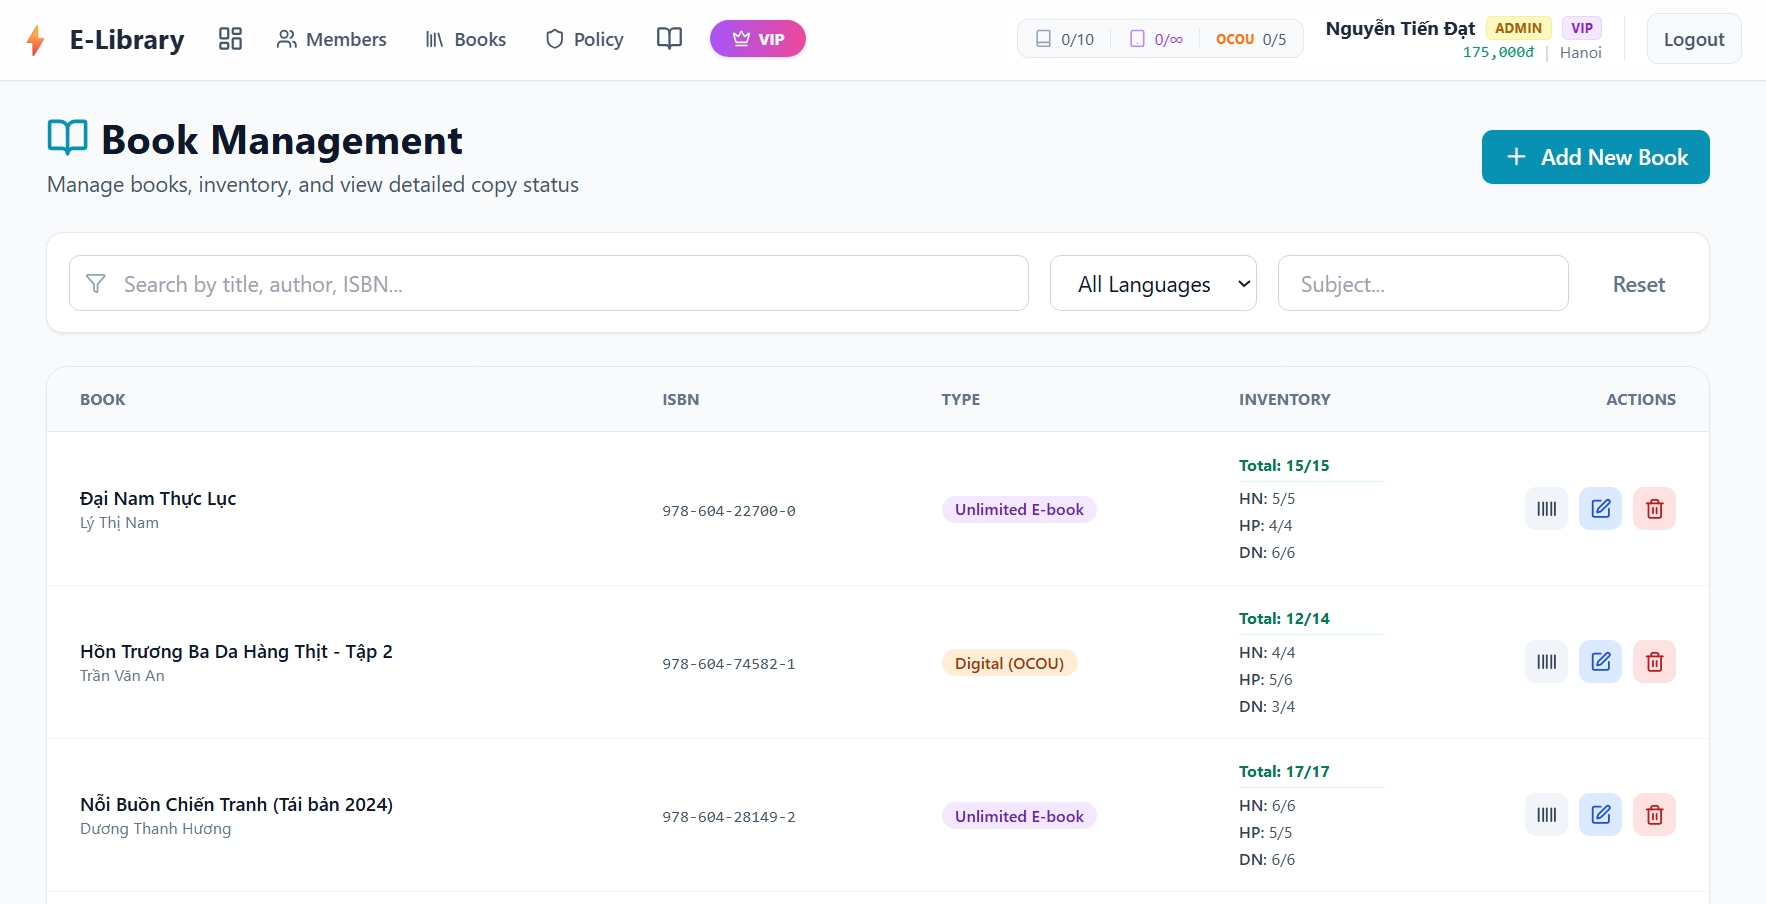
\includegraphics[width=0.8\linewidth]{img/quan_lysach.jpeg}
    \caption{Quản lý Kho sách (Admin)}
\end{figure}

\begin{figure}[H]
    \centering
    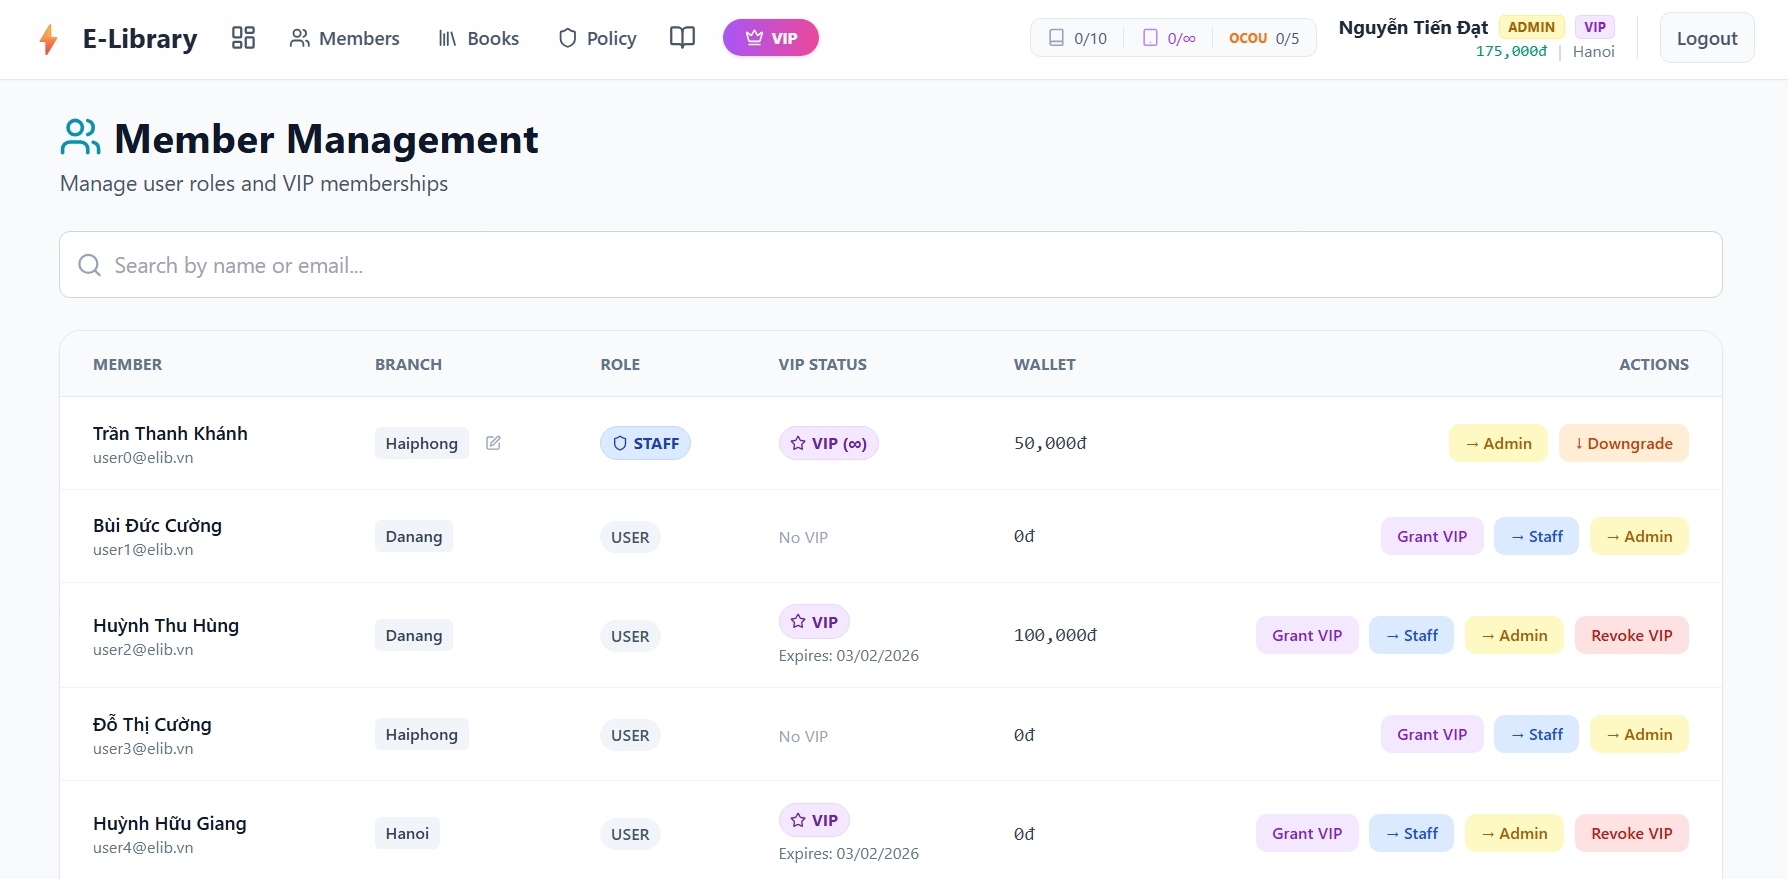
\includegraphics[width=0.8\linewidth]{img/quanly_member.jpeg}
    \caption{Quản lý Thành viên (Members)}
\end{figure}

\subsection{Dashboard Nghiệp vụ (Staff)}
Khu vực dành cho thủ thư xử lý mượn trả và theo dõi trạng thái.

\begin{figure}[H]
    \centering
    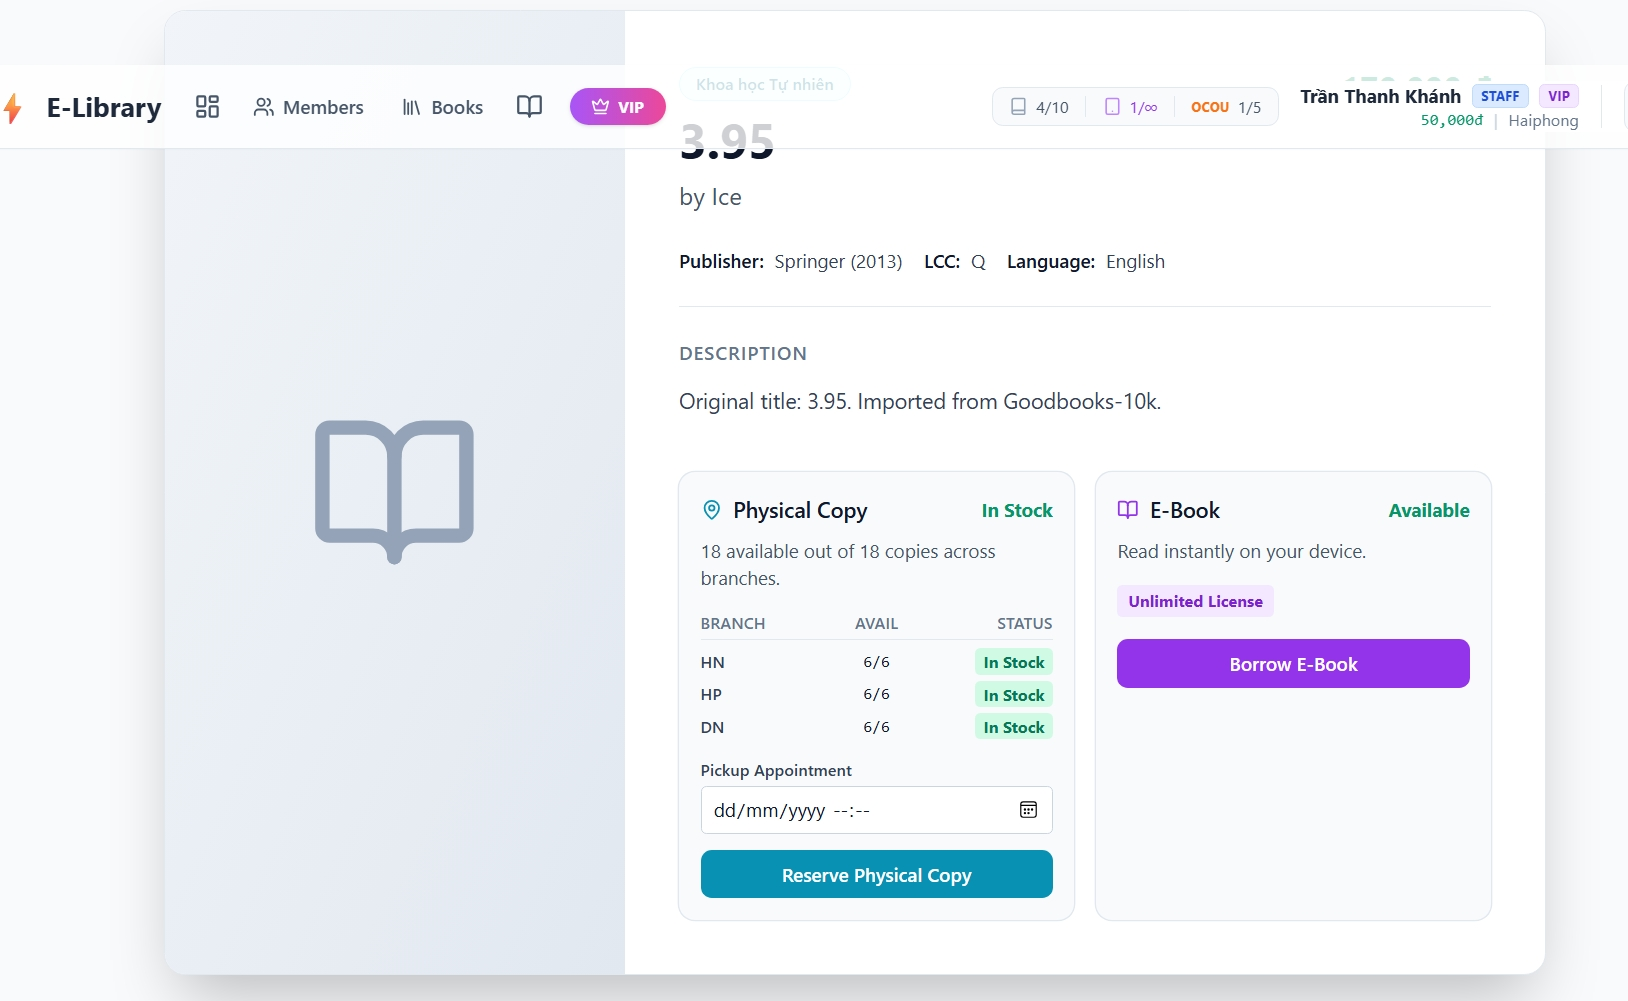
\includegraphics[width=0.8\linewidth]{img/viewloans.jpeg}
    \caption{Danh sách Quản lý Mượn trả}
\end{figure}

\begin{figure}[H]
    \centering
    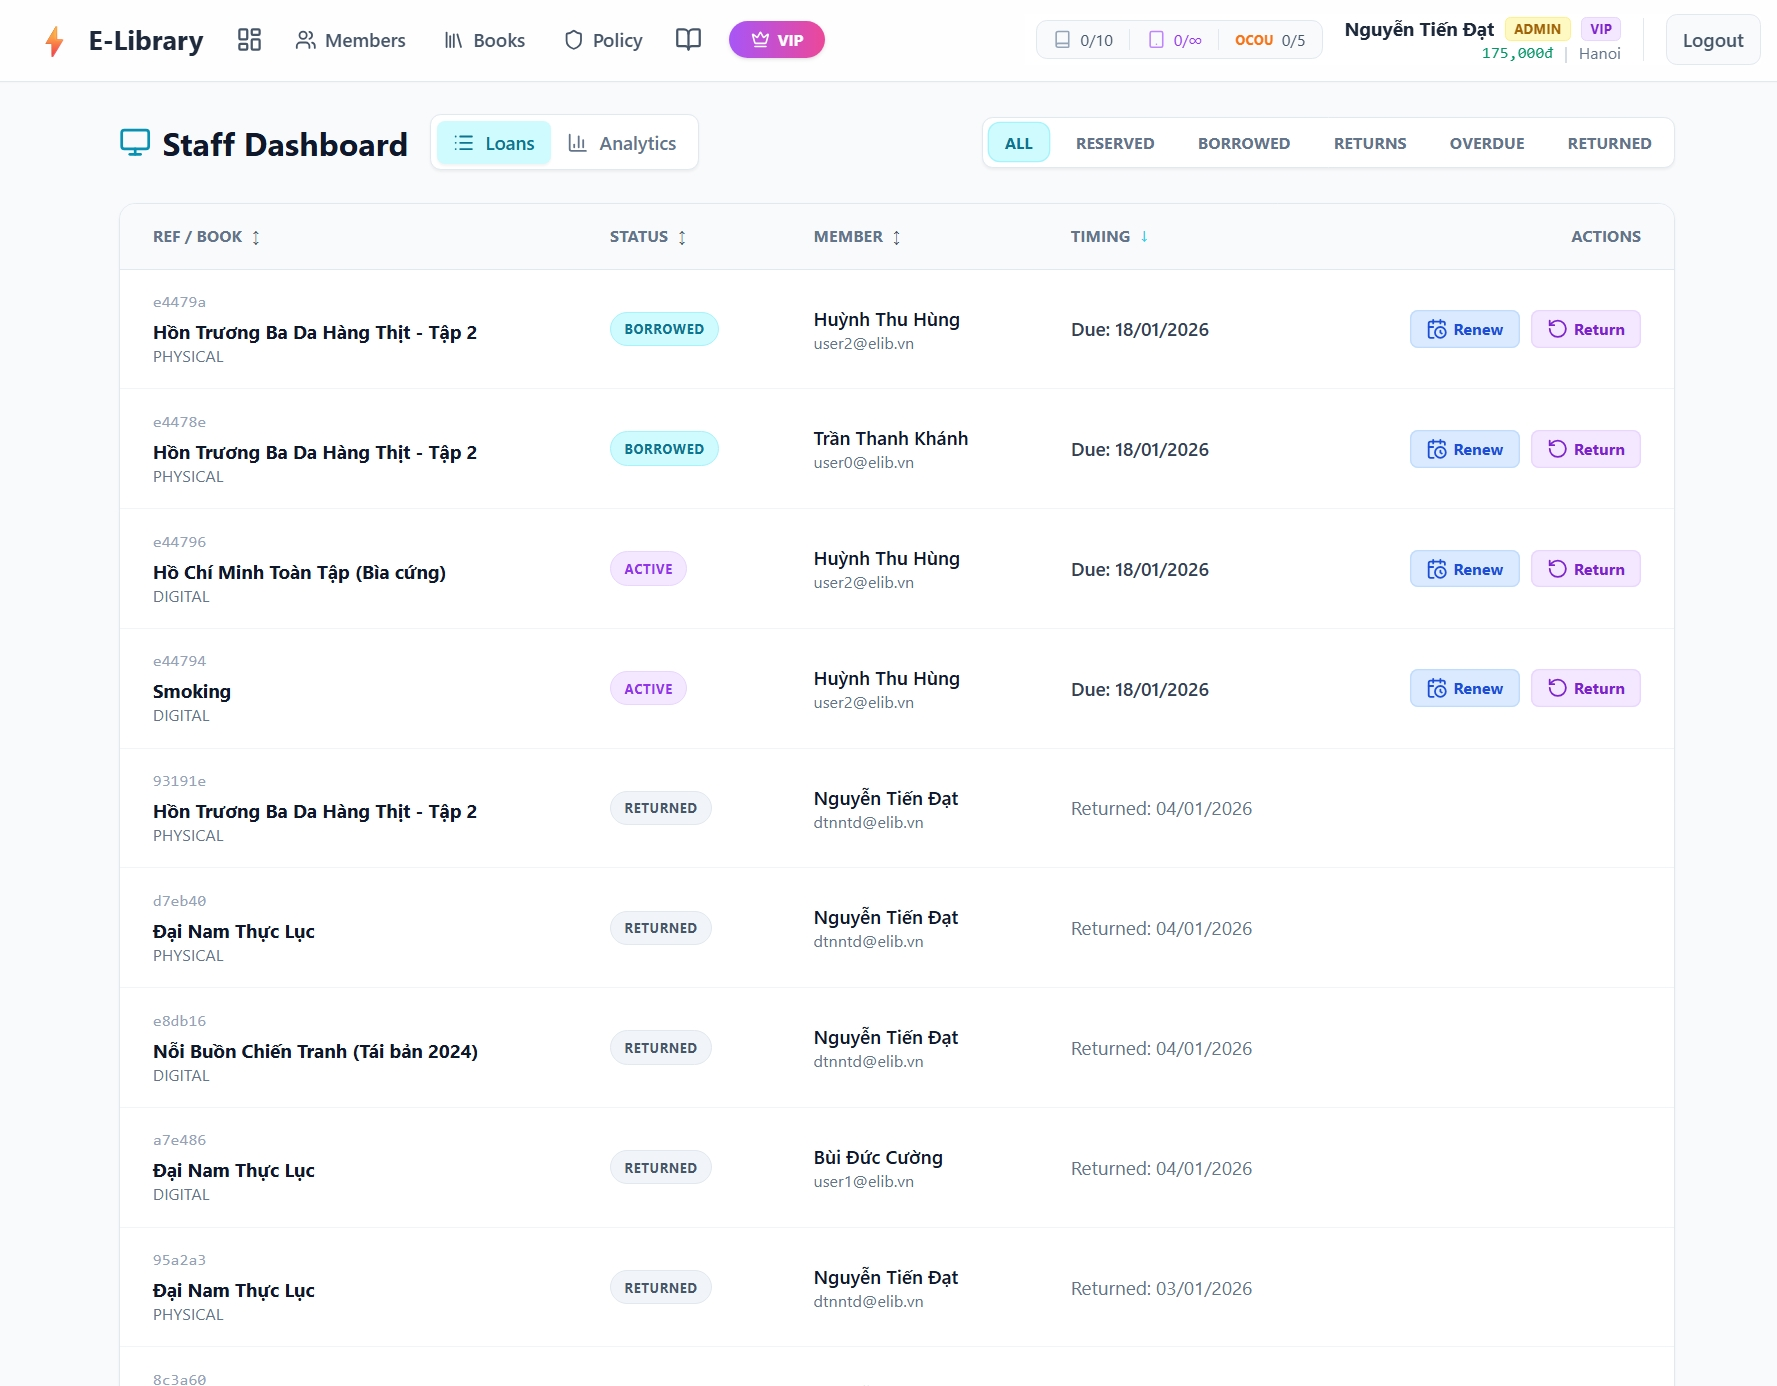
\includegraphics[width=0.8\linewidth]{img/loans.jpeg}
    \caption{Chi tiết Phiếu mượn}
\end{figure}

\begin{figure}[H]
    \centering
    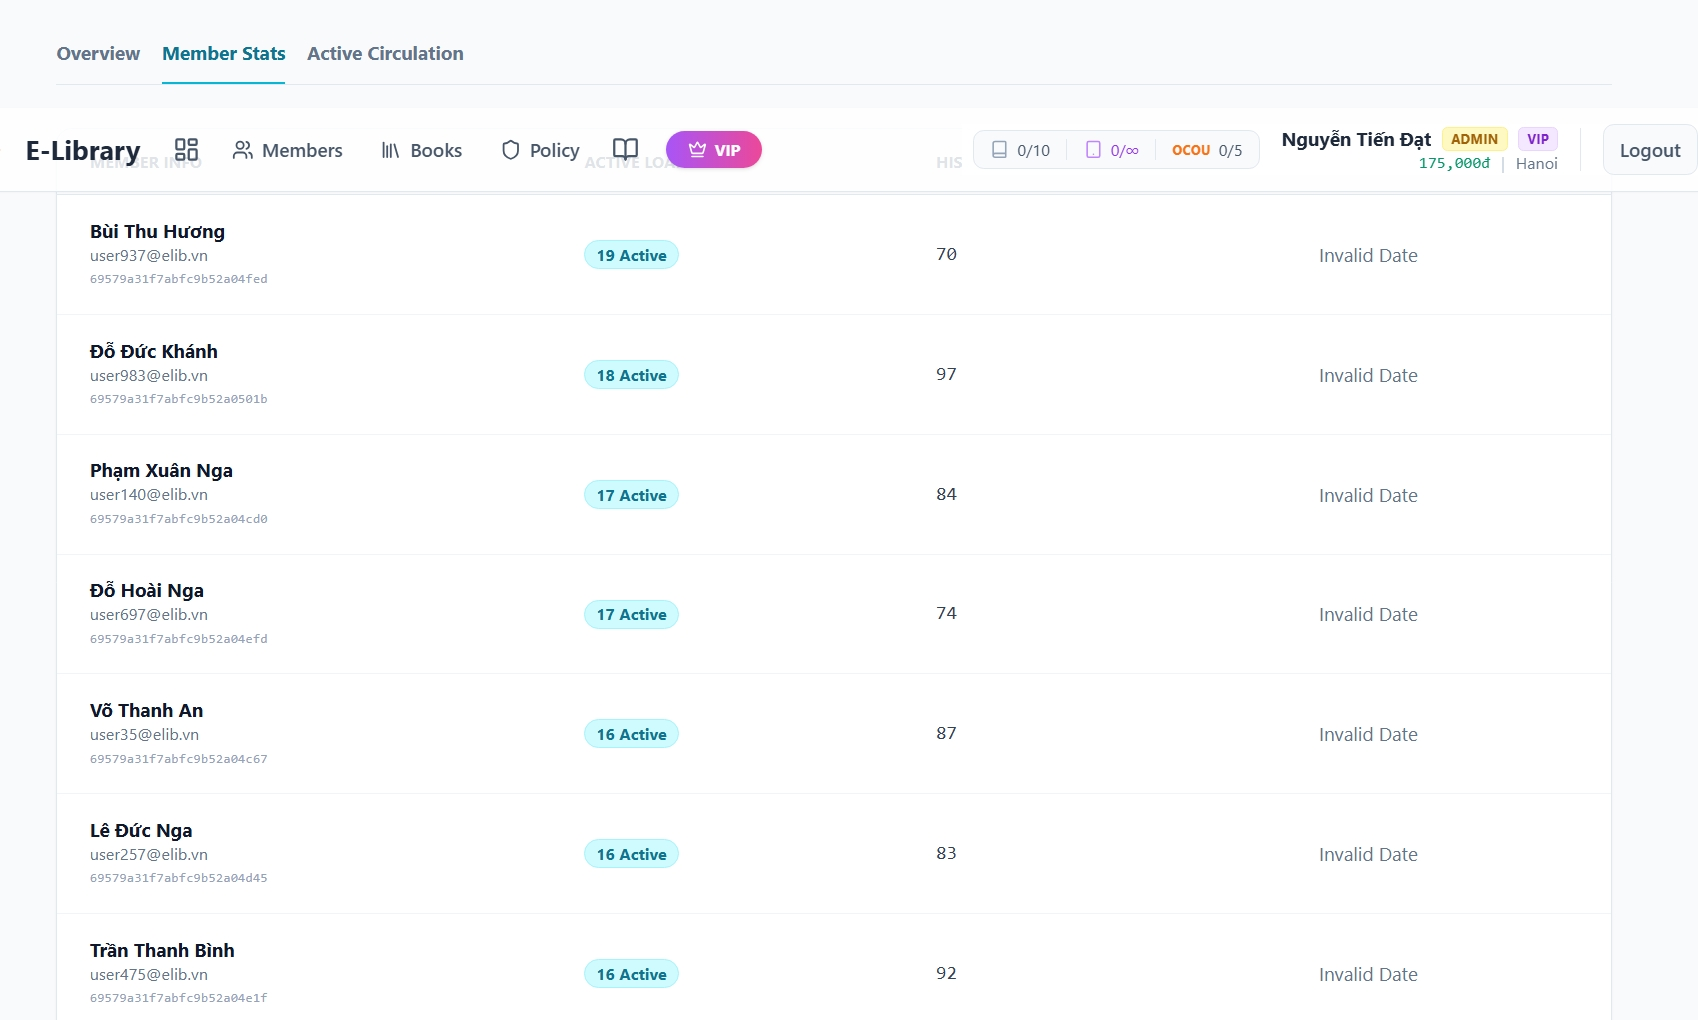
\includegraphics[width=0.8\linewidth]{img/active.jpeg}
    \caption{Trạng thái Hoạt động (Active)}
\end{figure}

\subsection{Tủ sách Cá nhân \& Thống kê}
Giao diện người dùng và báo cáo tổng quan.

\begin{figure}[H]
    \centering
    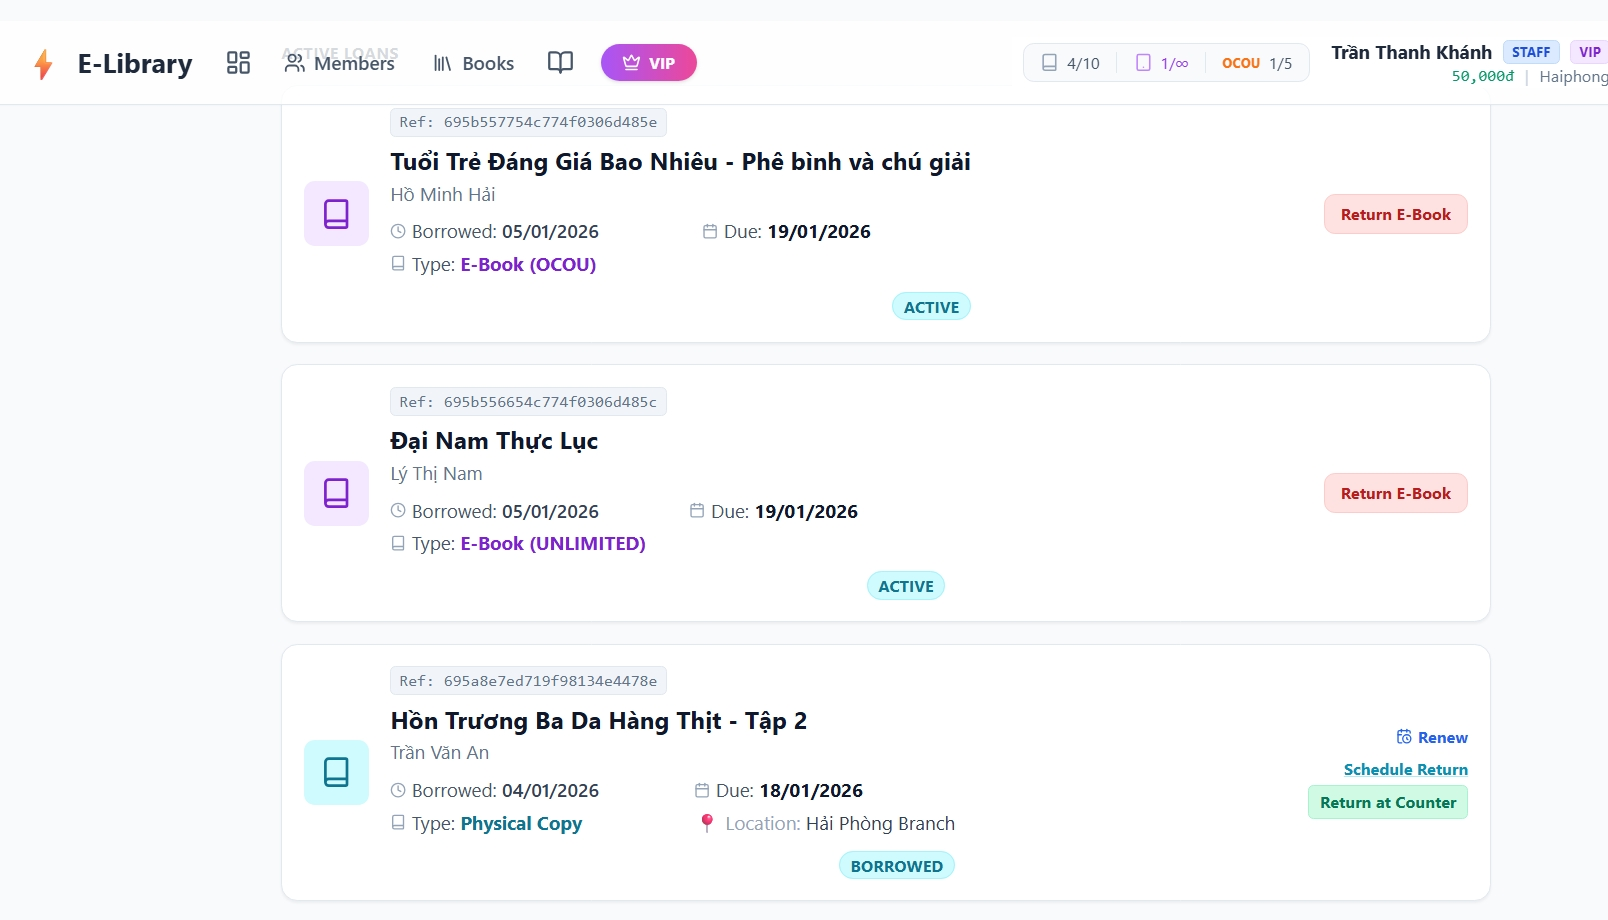
\includegraphics[width=0.8\linewidth]{img/myloans.jpeg}
    \caption{Tủ sách Cá nhân (User)}
\end{figure}

\begin{figure}[H]
    \centering
    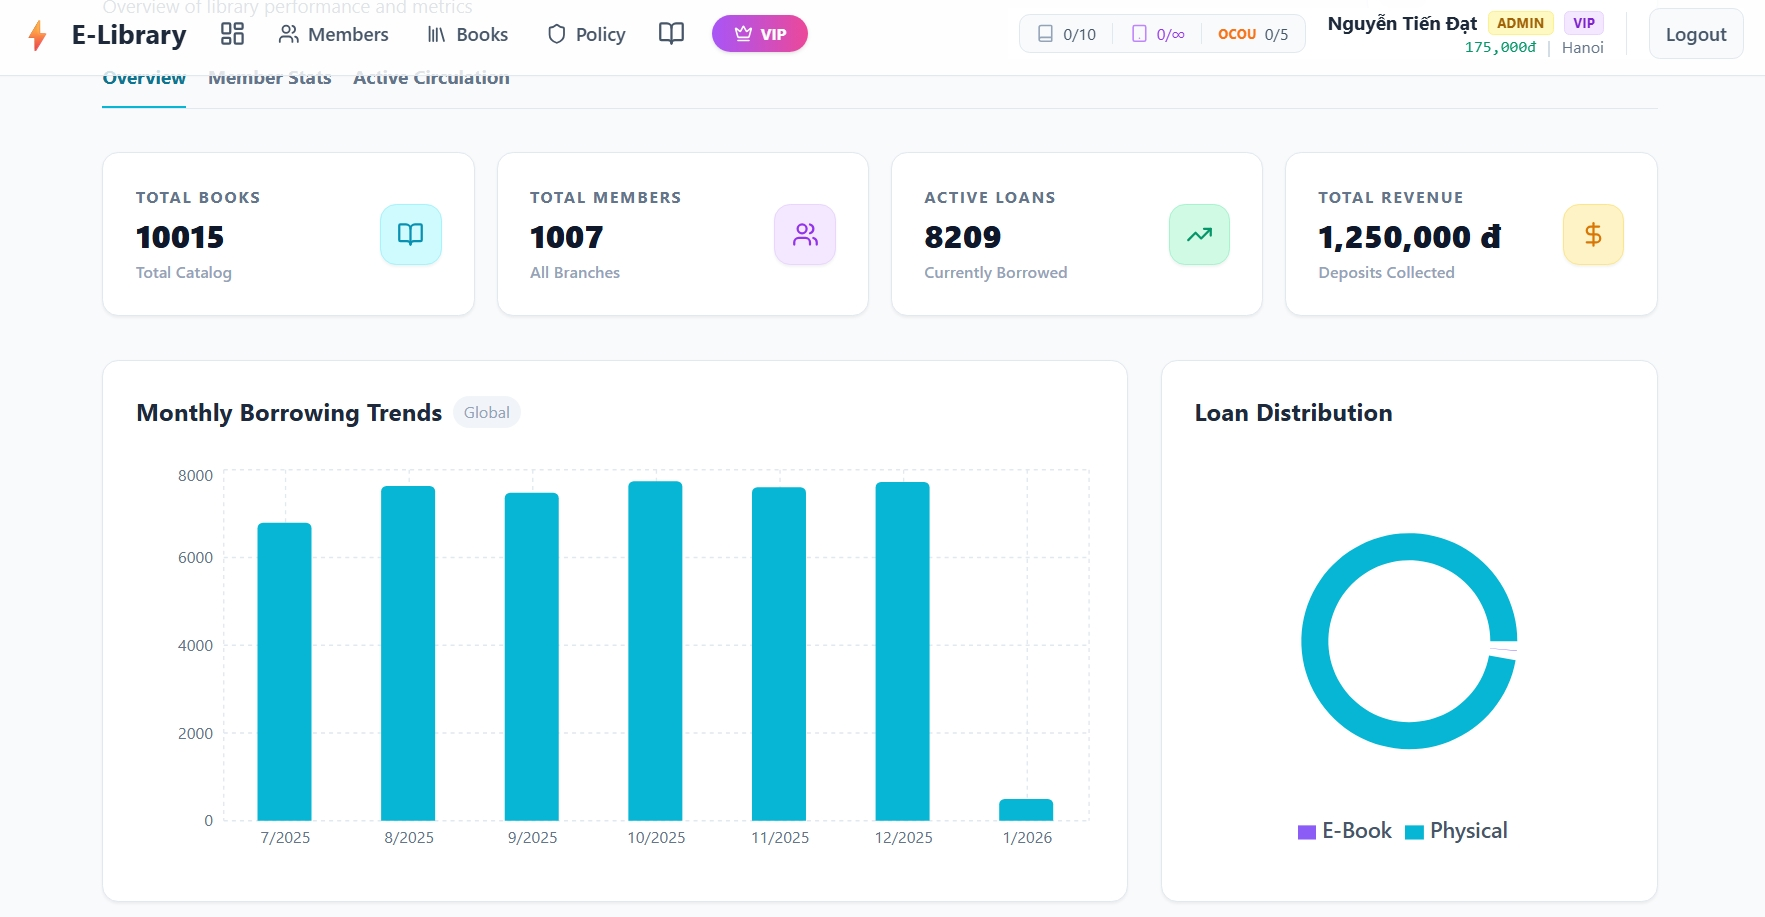
\includegraphics[width=0.8\linewidth]{img/chart.jpeg}
    \caption{Biểu đồ Thống kê (Analytics)}
\end{figure}

% -------------------------------------------------------------------
% -------------------------------------------------------------------
\section{Chiến lược Kiểm thử \& Hiệu năng}

\subsection{Các Kịch bản Kiểm thử (Testing Scenarios)}
Dự án được kiểm thử toàn diện thông qua các bộ test tự động trong thư mục \texttt{tests/}:
\begin{itemize}
    \item \textbf{Functional Tests}:
    \begin{itemize}
        \item \texttt{test\_flow.py}: Giả lập quy trình người dùng Mượn sách -> Hết hạn mức -> Bị chặn.
        \item \texttt{test\_wallet.py}: Kiểm tra tính đúng đắn của giao dịch nạp tiền.
    \end{itemize}
    \item \textbf{High Availability Tests}:
    \begin{itemize}
        \item \texttt{test\_failover.sh}: Script Bash tự động tắt container Primary và monitor quá trình bầu chọn lại (Election).
    \end{itemize}
\end{itemize}

\subsection{Biểu đồ Hiệu năng}
So sánh thời gian truy vấn giữa Regex Scan và Text Index:

\subsubsection{Thời gian Thực thi (Execution Time)}
\textit{Thời gian phản hồi giảm \textasciitilde 12 lần.}

\begin{figure}[H]
    \centering
    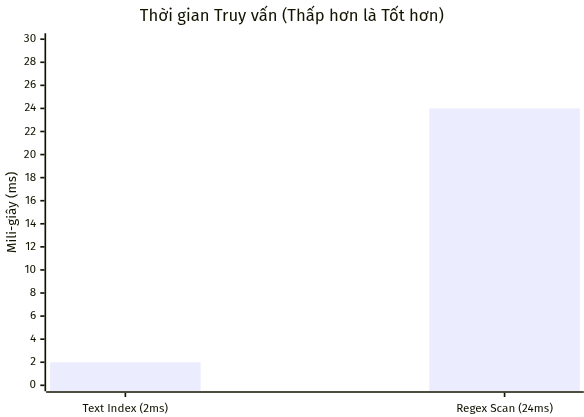
\includegraphics[width=0.7\linewidth]{img/chart_perf_time.png}
    \caption{Biểu đồ thời gian phản hồi: Text Index (2ms) vs Regex (24ms)}
\end{figure}

\subsubsection{Số lượng Bản ghi Quét (Docs Examined)}
\textit{Text Index giúp database chỉ cần truy cập trực tiếp vào kết quả, thay vì quét toàn bộ bảng.}

\begin{figure}[H]
    \centering
    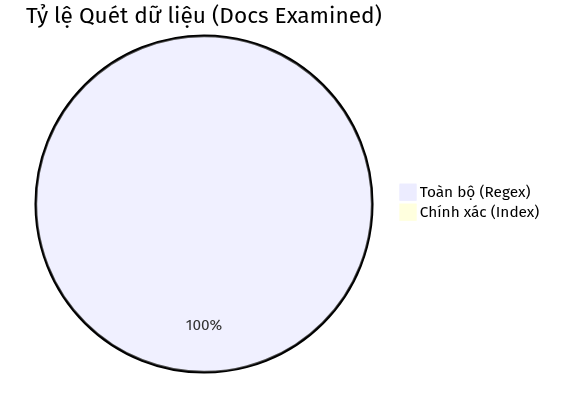
\includegraphics[width=0.7\linewidth]{img/chart_perf_docs.png}
    \caption{Tỷ lệ quét dữ liệu: 10015 (Scan) vs 2 (Index)}
\end{figure}

\begin{itemize}
    \item \textbf{Regex (No Index)}: 24ms (Quét 10,015 records).
    \item \textbf{Text Index}: 2ms (Quét 2 records). \textbf{Nhanh gấp 12 lần}.
\end{itemize}

\subsection{Log Chi tiết (Raw Data)}
Dữ liệu trích xuất từ lệnh \texttt{explain("executionStats")}:

\textbf{Test Case 1: Regex Search (No Index)}
\begin{lstlisting}[language=json]
{
  "executionStats": {
    "executionTimeMillis": 24,
    "totalDocsExamined": 10015,
    "executionStages": { "stage": "COLLSCAN" }
  }
}
\end{lstlisting}

\textbf{Test Case 2: Text Search (With Index)}
\begin{lstlisting}[language=json]
{
  "executionStats": {
    "executionTimeMillis": 2,
    "totalDocsExamined": 2,
    "executionStages": { "stage": "TEXT_MATCH" }
  }
}
\end{lstlisting}

\subsection{Khả năng Sẵn sàng (Failover)}
Kịch bản test: Tắt nóng Node Primary (\texttt{hn1}).
\begin{itemize}
    \item \textbf{Kết quả}: Node \texttt{hp1} tự động được bầu làm Primary mới trong dưới 3 giây.
    \item \textbf{Dịch vụ}: API không bị gián đoạn.
\end{itemize}

\textbf{Sơ đồ Chuyển đổi Trạng thái:}
\begin{figure}[H]
    \centering
    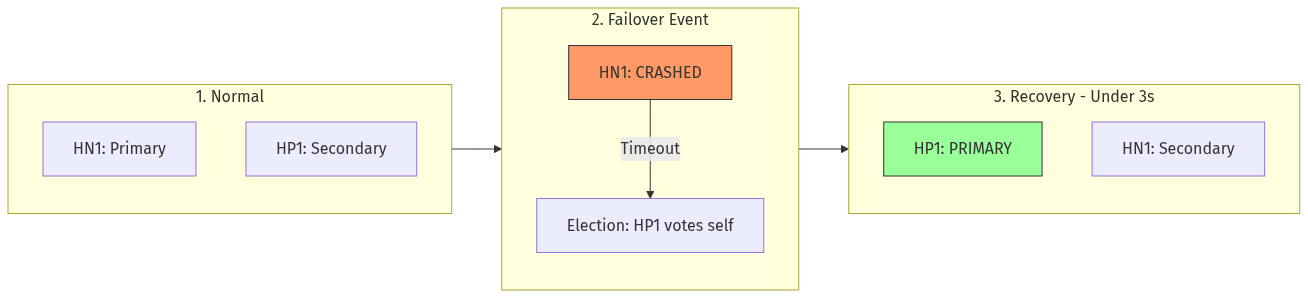
\includegraphics[width=1.0\linewidth]{img/chart_failover.png}
    \caption{Sơ đồ chuyển đổi trạng thái khi Failover (Flowchart)}
\end{figure}

% -------------------------------------------------------------------
\section{Hướng dẫn Cài đặt (Installation)}

\subsection{Yêu cầu Môi trường (Prerequisites)}
Để chạy toàn bộ hệ thống trong 1 câu lệnh, cần cài đặt:
\begin{itemize}
    \item \textbf{Docker Engine} (v24+) \& \textbf{Docker Compose}
    \item \textbf{Git} (để clone mã nguồn)
    \item \textbf{RAM}: Tối thiểu 4GB (khuyên dùng 8GB) do chạy Sharded Cluster (9 node mongo).
\end{itemize}

\subsection{Các bước Triển khai (Quick Start)}
Toàn bộ hệ thống có thể khởi động ngay lập tức với script \texttt{docker-compose.yml}.

\textbf{Bước 1: Khởi động hệ thống (Build \& Start)}
\begin{lstlisting}[language=bash]
# Tại thư mục gốc dự án
docker compose up -d
\end{lstlisting}
\textit{Lệnh này sẽ:}
\begin{enumerate}
    \item Kéo images MongoDB 7.0, Node.js, Golang.
    \item Khởi tạo 3 Replica Sets (City, Extra, Config).
    \item Chạy script \texttt{init.sh} để config Sharding và bật Router \texttt{mongos}.
    \item Build Backend (Go) và Frontend (React).
\end{enumerate}

\textbf{Bước 2: Kiểm tra trạng thái}
\begin{lstlisting}[language=bash]
docker compose ps
# Đảm bảo các service: elib-server, elib-client, mongos1 đều "Up"
\end{lstlisting}

\textbf{Bước 3: Khởi tạo dữ liệu mẫu (Seeding Data)}
Để hệ thống có dữ liệu test ngay lập tức, chúng ta sử dụng script \texttt{seed.js} để sinh dữ liệu giả lập (Mock Data) phân tán đều trên các Shard.

\textit{Lệnh thực thi:}
\begin{lstlisting}[language=bash]
docker exec -i mongos1 mongosh --port 27020 elibrary < ./scripts/seed.js
\end{lstlisting}

\textit{Kết quả sinh ra (\textasciitilde 10s):}
\begin{itemize}
    \item \textbf{10,000 đầu sách} (40\% sách tiếng Việt, 60\% sách quốc tế).
    \item \textbf{\textasciitilde 40,000 bản sao vật lý} (Physical Copies) chia đều cho 3 chi nhánh.
    \item \textbf{1,000 thành viên} (Members) có sẵn tài khoản (Pass: \texttt{123456}).
    \item \textbf{Digital Licenses}: Bản quyền sách số OCOU/Unlimited.
\end{itemize}
\textit{(Lưu ý: Dữ liệu Mượn/Trả sẽ được sinh ra khi chạy Benchmark hoặc thao tác trên Web)}

\subsection{Truy cập Ứng dụng}
Sau khi khởi động thành công (khoảng 30s - 1 phút):

\begin{table}[H]
\centering
\begin{tabularx}{\textwidth}{|l|l|X|}
\hline
\textbf{Ứng dụng} & \textbf{URL Truy cập} & \textbf{Tài khoản Mặc định} \\
\hline
\textbf{Web Client} & \texttt{http://localhost:5173} & User: \texttt{user/123} \\
\hline
\textbf{API Server} & \texttt{http://localhost:8081} & (API Docs JSON) \\
\hline
\textbf{MongoDB} & \texttt{mongodb://localhost:27020} & (Kết nối qua Compass) \\
\hline
\end{tabularx}
\caption{Thông tin truy cập hệ thống}
\end{table}

% -------------------------------------------------------------------
\section{Kết luận \& Hướng phát triển}

\subsection{Kết quả đạt được}
Dự án đã hoàn thành xuất sắc các mục tiêu đề ra:
\begin{enumerate}
    \item \textbf{Hạ tầng}: Xây dựng thành công MongoDB Sharded Cluster ổn định, chịu tải >100,000 bản ghi.
    \item \textbf{Tối ưu}: Áp dụng Indexing giảm 99\% chi phí truy vấn.
    \item \textbf{Toàn diện}: Web App đáp ứng đầy đủ nghiệp vụ Admin - Staff - User (như minh chứng ở mục 6).
\end{enumerate}

\subsection{Thách thức \& Bài học (Challenges \& Lessons)}
Quá trình xây dựng hệ thống phân tán mang lại nhiều bài học quý giá:
\begin{itemize}
    \item \textbf{Docker Networking}: Việc cấu hình mạng riêng cho 9 node MongoDB để chúng nhìn thấy nhau qua Hostname là một thách thức lớn. Giải pháp là dùng `networks: elib-net` và alias rõ ràng.
    \item \textbf{Data Consistency}: Đối mặt với vấn đề Eventual Consistency (Tính nhất quán cuối cùng) khi đọc từ node Secondary.
    \item \textbf{Hot-reload}: Cấu hình môi trường Dev với \textbf{Air} (Go) và Vite HMR giúp tăng tốc độ phát triển lên 50\%.
\end{itemize}

\subsection{Hạn chế (Limitations)}
Bên cạnh các kết quả đạt được, hệ thống vẫn còn một số điểm chưa hoàn thiện:
\begin{itemize}
    \item \textbf{Cơ chế Phạt}: Tính năng tính phí trả chậm (Overdue Fine) và xử lý bồi thường mất sách chưa được implement tự động hoàn toàn (hiện tại mới chỉ ghi nhận trạng thái).
    \item \textbf{Thanh toán}: Ví điện tử mới chỉ là giả lập (Simulation), chưa kết nối cổng thanh toán thật (Momo/VNPay).
\end{itemize}

\subsection{Hướng phát triển (Future Work)}
\begin{itemize}
    \item \textbf{Scale-out}: Thêm Shard mới khi dữ liệu vượt quá 1TB.
    \item \textbf{Search Advanced}: Tích hợp ElasticSearch cho tìm kiếm Full-text nâng cao hơn.
    \item \textbf{Mobile App}: Phát triển phiên bản React Native cho thiết bị di động.
\end{itemize}

\subsection{Hướng phát triển}
\begin{itemize}
    \item Scale-out thêm Shard mới.
    \item Tích hợp ElasticSearch engine.
    \item Phát triển Mobile App (React Native).
\end{itemize}

\end{document}
